%% Copyright (c) 2015-2020, RTE (http://www.rte-france.com)
%% See AUTHORS.txt
%% All rights reserved.
%% This Source Code Form is subject to the terms of the Mozilla Public
%% License, v. 2.0. If a copy of the MPL was not distributed with this
%% file, you can obtain one at http://mozilla.org/MPL/2.0/.
%% SPDX-License-Identifier: MPL-2.0
%%
%% This file is part of Dynawo, an hybrid C++/Modelica open source time domain simulation tool for power systems.

\documentclass[a4paper, 12pt]{report}

%%  Copyright (c) 2015-2019, RTE (http://www.rte-france.com)
%%  See AUTHORS.txt
%%  All rights reserved.
%%  This Source Code Form is subject to the terms of the Mozilla Public
%%  License, v. 2.0. If a copy of the MPL was not distributed with this
%%  file, you can obtain one at http://mozilla.org/MPL/2.0/.
%%  SPDX-License-Identifier: MPL-2.0
%%
%%  This file is part of Dynawo, an hybrid C++/Modelica open source time domain
%%  simulation tool for power systems.


%%%%%%%%%%%%%%%%%%%%%%%%%%%%%%%%%%%%%%%%%%%
% Define text and document settings
%%%%%%%%%%%%%%%%%%%%%%%%%%%%%%%%%%%%%%%%%%%

\usepackage{lmodern} % Latin Modern fam­ily of fonts
\usepackage[english]{babel} % English

% Specify encoding
\usepackage[utf8]{inputenc} % Input
\usepackage[T1]{fontenc} % Output

% Document structure setup
\usepackage{titlesec} % To change chapter format
\setcounter{tocdepth}{3} % Add subsubsection in Content
\setcounter{secnumdepth}{3} % Add numbering for subsubsection
\setlength{\parindent}{0pt} % No paragraph indentation

% Avoid numbering starting at each chapter for figures
\usepackage{chngcntr}
\counterwithout{figure}{chapter}

% Change title format for chapter
\titleformat{\chapter}{\Huge\bf}{\thechapter}{20pt}{\Huge\bf}

% To add links on page number in Content and hide red rectangle on links
\usepackage[hidelinks, linktoc=all]{hyperref}
\usepackage[nottoc]{tocbibind} % To add biblio in table of content
\usepackage{textcomp} % For single quote
\usepackage{url} % Allow linebreaks in \url command
\usepackage{listings} % To add code samples

% Define typography
\usepackage{xspace}
\usepackage{dirtree}
\newcommand{\Dynawo}[0]{Dyna$\omega$o\xspace}

% Default listings parameters
\lstset
{
  aboveskip={1\baselineskip}, % A bit of space above
  backgroundcolor=\color{shadecolor}, % Choose the background color
  basicstyle={\ttfamily\footnotesize}, % Use font and smaller size \small \footnotesize
  breakatwhitespace=true, % Sets if automatic breaks should only happen at whitespace
  breaklines=true, % Sets automatic line breaking
  columns=fixed, % Nice spacing -> fixed / flexible
  mathescape=false, % Escape to latex false
  numbers=left, % Where to put the line-numbers
  numberstyle=\tiny\color{gray}, % The style that is used for the line-numbers
  showstringspaces=false, % Do not emphasize spaces in strings
  tabsize=4, % Number of spaces of a TAB
  texcl=false, % Activates or deactivates LaTeX comment lines
  upquote=true % Upright quotes
}

%%%%%%%%%%%%%%%%%%%%%%%%%%%%%%%%%%%%%%%%%%%
% Define plots settings
%%%%%%%%%%%%%%%%%%%%%%%%%%%%%%%%%%%%%%%%%%%

% Macro pack­age for cre­at­ing graph­ics
\usepackage{tikz}
\usepackage{subfigure}
\usepackage{float}

% Draws func­tion plots (based on pgf/tikz)
\usepackage{pgfplots}
\pgfplotsset{enlarge x limits=false, xlabel={\begin{small}$time$ (s)\end{small}}, height=0.6\textwidth, width=1\textwidth}
\pgfplotstableset{col sep=semicolon}

% Define colors
\usepackage{color}
\definecolor{blue}{rgb}{.3,.5,1}
\definecolor{deepblue}{rgb}{0,0,1}
\definecolor{darkblue}{rgb}{0,0,.4}
\definecolor{red}{rgb}{1,0,0}
\definecolor{darkred}{rgb}{.56,0,0}
\definecolor{pink}{rgb}{.933,0,.933}
\definecolor{purple}{rgb}{0.58,0,0.82}
\definecolor{green}{rgb}{0.133,0.545,0.133}
\definecolor{darkgreen}{rgb}{0,.4,0}
\definecolor{gray}{rgb}{.3,.3,.3}
\definecolor{darkgray}{rgb}{.2,.2,.2}
\definecolor{shadecolor}{gray}{0.925}

%%%%%%%%%%%%%%%%%%%%%%%%%%%%%%%%%%%%%%%%%%%
% Define blocks for simple network drawings
%%%%%%%%%%%%%%%%%%%%%%%%%%%%%%%%%%%%%%%%%%%

% Define blocks for newtorks drawings
\usepackage{amsmath} % Add math­e­mat­i­cal fea­tures
\usepackage{schemabloc} % Add block diagram library (french one)

%% Define infinite bus
\tikzset{infinite bus/.pic={
  code={
  \draw (0,0) circle (2) node[inner sep=0, outer sep=0] {{$\infty$}};
  \draw (2,0) --++ (2,0);
  }
  }
}

%% Define transformer
\tikzset{transfo/.pic={
  code={
  \draw (0,0) circle (2);
  \draw (2,0) circle (2);
  \draw (4,0) --++ (4,0);
  \draw (-2,0) --++ (-4,0);
  }
  }
}

%% Define generator
\tikzset{generator/.pic={
  code={
    \draw (0,0) circle (2);
    \draw (0,0) arc (0:180:0.5);
    \draw (0,0) arc (180:360:0.5);
    \draw (-2,0) --++ (-2,0);
  }
  }
}

%% Define generator controls
\tikzset{VR/.pic={
  code={
  \draw (0,0) circle (2) node[inner sep=0, outer sep=0] {{VR}};
  }
  }
}

%% Define SVarC
\tikzset{SVarC/.pic={
  code={
  \draw (0,0) circle (4) node[inner sep=0, outer sep=0] {{SVarC}};
  }
  }
}
\pgfkeys{
/pgf/number format/read comma as period
}

\begin{document}

\title{DynaSwing use examples}
\date\today

\maketitle
\tableofcontents

\chapter{Impact of the excitation control on a synchronous generator transient stability - Kundur Example 13.2}

This test case is inspired by example 13.2 of Kundur "Power System Stability and Control" book.

% Generic description of the non regression test
% List of scenarios
\section{Test case description}

This test case compares the behavior of a synchronous machine subject to a 3-phase fault with three different excitation controls:
\begin{itemize}
\item a set-point;
\item a proportional voltage regulator;
\item a proportional voltage regulator with a PSS function;
\end{itemize}
To do so, a simple Synchronous Machine - Infinite Bus (SMIB) system is used. It consists of a single machine connected to the infinite bus through two parallel lines and a transformer as presented in Figure 1.

\begin{figure}[H]
\centering
\def\factor{0.4}
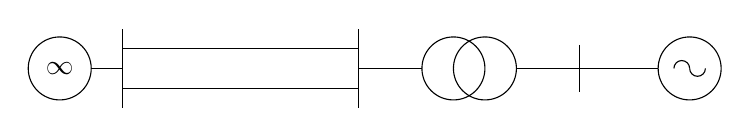
\begin{tikzpicture}[every node/.style={inner sep=0,outer sep=0}]
% Infinite bus
\path (0,0)  pic[scale=0.2,local bounding box=bus] {infinite bus};
%% Transfo
\path (5,0) pic[scale=0.2,local bounding box=transfo] {transfo};
% Generator
\path (8,0) pic[scale=0.2,local bounding box=gen] {generator};
% Line 1
\draw ([yshift=0.25cm]bus.east) -- ([yshift=0.25cm]transfo.west);
% Line 1
\draw ([yshift=-0.25cm]bus.east) -- ([yshift=-0.25cm]transfo.west);
% Bus inf
\draw (bus.east) ++ (0,0.5) --++ (0,-1);
% Bus tfo 1
\draw (transfo.west) ++ (0,0.5) node (bustop) {} --++ (0,-1) node (busbottom) {};
% Bus tfo 2
\draw (transfo.east) ++ (0,0.3) node (bustop) {} --++ (0,-0.6) node (busbottom) {};
% Transfo-Generator connection
\draw (transfo.east) -- (gen.west);
\end{tikzpicture}
\caption{SMIB system representation}
\label{circuit-1}
\end{figure}

The SMIB system is a well-known test case in the power system community. It is very often used to illustrate the transient or the small-signal stability of a synchronous machine. It is also used to demonstrate the behavior of a new regulation, such as a speed governor, a voltage regulation or a power-system stabilizer.

\textbf{Note. As compilation at run-time is utilized for this example, the simulation time for each test case is around 1' with 95\% of the time spent in the Modelica models compilation. For industrial simulations, the idea is to only use black box models as in the IEEE14 and IEEE57 examples that run in a much faster way.}

\subsection{Initial Conditions}

The infinite bus base voltage is 400 kV and the synchronous machine base voltage is 24 kV. \\

The generator is a 2220 MVA equivalent for four 555 MVA generators.\\

The lines and transformer parameters in per unit on 100 MVA base are:
\begin{center}
\begin{tabular}{l|l|l}
   $R_1=0$ & $R_2=0$ & $R_{Tfo}=0$ \\
   $X_1=0.022522$ & $X_2=0.04189$ & $X_{Tfo}=0.00675$ \\
\end{tabular}
\end{center}

The reference angle for the load flow is set at the infinite bus, and the voltage amplitude at the machine terminal is set to 1. \\

The load flow results in per unit on 100 MVA base are:
\begin{center}
\begin{tabular}{l|l|l}
   $U_{Inf}=0.90081$ & $U_{SM}=1$ & $P_{SM}=19.98$ \\
   $\Theta_{Inf}=0rad$ & $\Theta_{SM}=0.49445rad$ & $Q_{SM}=9.68$ \\
\end{tabular}
\end{center}

\subsection{Models}

The equivalent generator parameters are given in per unit on 2220 MVA - 24 kV (no transformer included, no saturation):
\begin{center}
\begin{tabular}{l|l|l|l}
   $R_a=0.003$ & $X_l=0.15$ & $H=3.5$ & $D=0$ \\
   $X_d=1.81$ & $T'_d0=8s$ & $X_q=1.76$ & $T'_q0=1s$ \\
   $X'_d=0.30$ & $T''_d0=0.03s$ & $X'_q=0.65$ & $T''_q0=0.07s$ \\
   $X''_d=0.23$ & & $X''_q=0.25$ &  \\
\end{tabular}
\end{center}

The system reference frequency omegaRef is set to 1.\\
The machine is under constant mechanical power. \\
The voltage regulator is as follows:
\begin{figure}[H]
\centering
\begin{tikzpicture}
\sbEntree{E}
\sbBloc[3]{Transducer}{$\dfrac{1}{1+s\cdot T_R}$}{E}
\sbRelier[$U_S$]{E}{Transducer}
\sbCompSum[5]{errAVR}{Transducer}{+}{+}{-}{}
\sbRelier{Transducer}{errAVR}
\sbDecaleNoeudy[-4]{errAVR}{Uc}
\sbRelier[$U_C$]{Uc}{errAVR}
\sbBloc{Exciter}{$K_A$}{errAVR}
\sbRelier{errAVR}{Exciter}
\sbBlocL{Limiter}{\tikz {\draw (-0.4,-0.4) -- (0,-0.4);\draw (0,-0.4) -- (0,0.4); \draw (0,0.4) -- (0.4,0.4); }}{Exciter}
\sbSortie[5]{S}{Limiter}
\sbRelier[$Efd$]{Limiter}{S}
\sbDecaleNoeudy[4]{errAVR}{VPSS}
\sbRelier[$V_{PSS}$]{VPSS}{errAVR}
\end{tikzpicture}
\caption{Voltage regulator}
\end{figure}

The signal $V_{PSS}$ is set to zero if no PSS is used.


The voltage regulator parameters are:
\begin{center}
\begin{tabular}{l|l}
   $K_A=200$ & $Efd_{Max}=7$  \\
   $T_R=0.015s$ & $Efd_{Min}=-6.4$   \\
\end{tabular}
\end{center}

A PSS is used in one of the test, in order to see its influence on the synchronous machine transient stability. Its structure is as follows:
\begin{figure}[H]
\centering
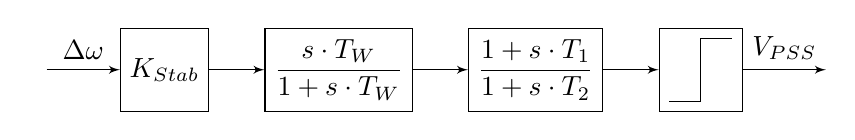
\begin{tikzpicture}
\sbEntree{E}
\sbBloc[3]{Gain}{$K_{Stab}$}{E}
\sbRelier[$\Delta \omega$]{E}{Gain}
\sbBloc{Washout}{$\dfrac{s\cdot T_W}{1+s\cdot T_W}$}{Gain}
\sbRelier{Gain}{Washout}
\sbBloc{PhaseCompensation}{$\dfrac{1+s\cdot T_1}{1+s\cdot T_2}$}{Washout}
\sbRelier{Washout}{PhaseCompensation}
\sbBlocL{LimiterPSS}{\tikz {\draw (-0.4,-0.4) -- (0,-0.4);\draw (0,-0.4) -- (0,0.4); \draw (0,0.4) -- (0.4,0.4); }}{PhaseCompensation}
\sbSortie[3]{S}{LimiterPSS}
\sbRelier[$V_{PSS}$]{LimiterPSS}{S}
\end{tikzpicture}
\caption{Power System Stabilizer structure}
\end{figure}

The power system stabilizer parameters are:
\begin{center}
\begin{tabular}{l|l|l}
   $K_{Stab}=9.5$ & $T_1=0.154s$ & $Vs_{Max}=0.2$  \\
   $T_W=1.41s$ & $T_2=0.033s$ & $Vs_{Min}=-0.2$   \\
\end{tabular}
\end{center}

\subsection{Scenario}
The simulated scenario is :
\begin{itemize}
\item at $t=1s$: a 0.07s three-phase fault at the transformer high voltage terminal;
\item at $t=1.07s$: the opening of line 2;
\end{itemize}

\subsection{Solver}
The solver used is the variable time step solver IDA with the following parameters:
\begin{itemize}
\item $Order$=2;
\item $Accuracy_{Rel}$=$10^{-4}$;
\item $Accuracy_{Abs}$=$10^{-4}$;
\end{itemize}

\section{Results}

The results of the simulations performed with the different excitation controls are presented bellow. Here are the different observations:
\begin{itemize}
\item with a constant excitation voltage, the system remains stable but the level of the oscillations damping is low;
\item with the proportional voltage regulator, the system loses synchronism in the third swing. The regulator's gain is very high and the control acts to fast, it destabilizes the system;
\item with the proportional voltage including a PSS function, the system remains stable and the oscillations are very well damped. We see here the positive impact of the PSS on the machine's stability;
\end{itemize}

These results match the results obtained in the example 13 of the "Power System Stability and Control" book of P.Kundur.

\begin{figure}[H]
  \caption{Rotor angle (deg)}
  \begin{tikzpicture}
    \begin{axis} [ymin = 0, ymax = 3.14, legend style={at={(0.5,-0.1)},anchor=north}]
        \addplot[color=red!50]
        table[x=time, y=SM_gen_theta]
        {../Kundur_Example13/reference/outputs_AVR_SetPoint/curves/curves.csv};
        \addplot[color=blue!50]
        table[x=time, y=SM_gen_theta]
        {../Kundur_Example13/reference/outputs_AVR_NoPSS/curves/curves.csv};
        \addplot[color=green!50]
        table[x=time, y=SM_gen_theta]
        {../Kundur_Example13/reference/outputs_AVR_PSS/curves/curves.csv};
        \legend{$SetPoint$, $AVRNoPSS$, $AVRWithPSS$}
    \end{axis}
  \end{tikzpicture}
\end{figure}

\begin{figure}[H]
  \caption{Stator voltage (pu)}
  \begin{tikzpicture}
    \begin{axis}[legend style={at={(0.5,-0.1)},anchor=north}]
        \addplot[color=red!50]
        table[x=time, y=SM_gen_UPu]
        {../Kundur_Example13/reference/outputs_AVR_SetPoint/curves/curves.csv};
        \addplot[color=blue!50]
        table[x=time, y=SM_gen_UPu]
        {../Kundur_Example13/reference/outputs_AVR_NoPSS/curves/curves.csv};
        \addplot[color=green!50]
        table[x=time, y=SM_gen_UPu]
        {../Kundur_Example13/reference/outputs_AVR_PSS/curves/curves.csv};
        \legend{$SetPoint$, $AVRNoPSS$, $AVRWithPSS$}
    \end{axis}
  \end{tikzpicture}
\end{figure}

\begin{figure}[H]
  \caption{Active power (pu)}
  \begin{tikzpicture}
    \begin{axis} [ymin = 0, legend style={at={(0.5,-0.1)},anchor=north}]
        \addplot[color=red!50]
        table[x=time, y=SM_gen_PGenPu]
        {../Kundur_Example13/reference/outputs_AVR_SetPoint/curves/curves.csv};
        \addplot[color=blue!50]
        table[x=time, y=SM_gen_PGenPu]
        {../Kundur_Example13/reference/outputs_AVR_NoPSS/curves/curves.csv};
        \addplot[color=green!50]
        table[x=time, y=SM_gen_PGenPu]
        {../Kundur_Example13/reference/outputs_AVR_PSS/curves/curves.csv};
        \legend{$SetPoint$, $AVRNoPSS$, $AVRWithPSS$}
    \end{axis}
  \end{tikzpicture}
\end{figure}

\chapter{ENTSO-E Controller Test Report}

These three test cases are the ones used in an ENTSO-E work conducted to compare different transient simulation tools responses on a single machine infinite bus. The different test cases and the models used are presented in the ENTSO-E report called "Documentation on Controller Tests in Test Grid Configurations" available online at \url{https://eepublicdownloads.entsoe.eu/clean-documents/pre2015/publications/entsoe/RG_SOC_CE/131127_Controller_Test_Report.pdf}.\\

\textbf{Note. As compilation at run-time is utilized for test cases 1 and 2, the simulation time for each test case is around 1' with 95\% of the time spent in the Modelica models compilation. For test case 3, only blackbox models are used and the simulation time is around 1 s, as one could expect for such a test case.}

\section{Test case description}

\subsection{Scenario}

The scenarios considered are the following ones:

\begin{center}
  \resizebox{\textwidth}{!}{
\begin{tabular}{|c|c|c|}
  \hline
  Test Case & Network & Event \\
  \hline
  1 & Generator Only & Voltage reference step \\
  2 & Generator and Load & Active power variation on the load \\
  3 & SMIB & Three-phase short circuit at the transformer high-level side \\
  \hline
\end{tabular} }
\end{center}

\subsection{Solver}

The solver used for these simulations is the variable time step solver IDA with the following main parameters:
\begin{itemize}
\item $Order$=2;
\item $Accuracy_{Rel}$=$10^{-6}$;
\item $Accuracy_{Abs}$=$10^{-6}$;
\end{itemize}

\section{Results}

The results obtained perfectly match the ones presented in the report and demonstrate DynaSwing accuracy.

\subsection{Test Case 1}

The purpose of the first test case is to compare the dynamic behaviour of the model for the synchronous machine and its AVR by analysing the terminal voltage and the excitation voltage inside the machine. These variables evolutions are identical to the ones reported in the reference document.

\begin{figure}[H]
\subfigure[Terminal voltage]
{%
  \begin{tikzpicture}
    \begin{axis}[height = 2in]
        \addplot[color=blue!50]
        table[x=time,y=SynchronousGenerator_generator_UPu]
        {../ENTSOE/TestCase1/reference/outputsTestCase1/curves/curves.csv};
    \end{axis}
  \end{tikzpicture}
}
\subfigure[Excitation voltage]
{%
  \begin{tikzpicture}
    \begin{axis}[height = 2in]
        \addplot[color=blue!50]
        table[x=time, y=SynchronousGenerator_generator_efdPu]
        {../ENTSOE/TestCase1/reference/outputsTestCase1/curves/curves.csv};
    \end{axis}
  \end{tikzpicture}
}
\caption{Test Case 1 Results}
\end{figure}

\subsection{Test Case 2}

The purpose of the second test case is to compare the dynamic behaviour of the model for the synchronous generator and its governor by analysing the terminal voltage, the active and mechanical power of the synchronous machine, the reactive power of the synchronous machine and the speed. The results got with DynaSwing match the ones presented in the official report.

\begin{figure}[H]
\subfigure[Terminal voltage]
{%
  \begin{tikzpicture}
    \begin{axis}[height = 1.5in, yticklabel style={/pgf/number format/.cd,fixed,precision=3}]
        \addplot[color=blue!50]
        table[x=time,y=SynchronousGenerator_generator_UPu]
        {../ENTSOE/TestCase2/reference/outputsTestCase2/curves/curves.csv};
    \end{axis}
  \end{tikzpicture}
}
\subfigure[Active power]
{%
  \begin{tikzpicture}
    \begin{axis}[height = 1.5in]
        \addplot[color=blue!50]
        table[x=time, y expr=\thisrow{SynchronousGenerator_generator_PGenPu}/4.75]
        {../ENTSOE/TestCase2/reference/outputsTestCase2/curves/curves.csv};
    \end{axis}
  \end{tikzpicture}
}
\subfigure[Mechanical power]
{%
  \begin{tikzpicture}
    \begin{axis}[height = 1.5in]
        \addplot[color=blue!50]
        table[x=time, y expr=\thisrow{SynchronousGenerator_generator_PmPu}]
        {../ENTSOE/TestCase2/reference/outputsTestCase2/curves/curves.csv};
    \end{axis}
  \end{tikzpicture}
}
\subfigure[Speed]
{%
  \begin{tikzpicture}
    \begin{axis}[height = 1.5in, yticklabel style={/pgf/number format/.cd,fixed,precision=3}]
        \addplot[color=blue!50]
        table[x=time, y expr=\thisrow{SynchronousGenerator_generator_omegaPu}]
        {../ENTSOE/TestCase2/reference/outputsTestCase2/curves/curves.csv};
    \end{axis}
  \end{tikzpicture}
}
\caption{Test Case 2 Results}
\end{figure}

\subsection{Test Case 3}

The purpose of the third test case is to compare the dynamic behaviour of the model for the synchronous machine with its whole control in operation during and after a three-phase short-circuit by analysing the terminal voltage, the excitation voltage inside the generator, the active and reactive power of the synchronous machine as well as speed. The results obtained prove the good behavior of DynaSwing.

\begin{figure}[H]
\subfigure[Terminal voltage]
{%
  \begin{tikzpicture}
    \begin{axis}
        \addplot[color=blue!50]
        table[x=time,y=SynchronousGenerator_generator_UPu]
        {../ENTSOE/TestCase3/reference/outputsTestCase3/curves/curves.csv};
    \end{axis}
  \end{tikzpicture}
}
\subfigure[Excitation voltage]
{%
  \begin{tikzpicture}
    \begin{axis}
        \addplot[color=blue!50]
        table[x=time,y=SynchronousGenerator_generator_UPu]
        {../ENTSOE/TestCase3/reference/outputsTestCase3/curves/curves.csv};
    \end{axis}
  \end{tikzpicture}
}
\end{figure}

\begin{figure}[H]
\subfigure[Active power]
{%
  \begin{tikzpicture}
    \begin{axis}
        \addplot[color=blue!50]
        table[x=time, y expr=\thisrow{SynchronousGenerator_generator_PGenPu}/4.75]
        {../ENTSOE/TestCase3/reference/outputsTestCase3/curves/curves.csv};
    \end{axis}
  \end{tikzpicture}
}
\subfigure[Reactive power]
{%
  \begin{tikzpicture}
    \begin{axis}
        \addplot[color=blue!50]
        table[x=time, y expr=\thisrow{SynchronousGenerator_generator_QGenPu}/1.56]
        {../ENTSOE/TestCase3/reference/outputsTestCase3/curves/curves.csv};
    \end{axis}
  \end{tikzpicture}
}
\end{figure}

\begin{figure}[H]
\subfigure[Speed]
{%
  \begin{tikzpicture}
    \begin{axis}
        \addplot[color=blue!50]
        table[x=time, y=SynchronousGenerator_generator_omegaPu]
        {../ENTSOE/TestCase3/reference/outputsTestCase3/curves/curves.csv};
    \end{axis}
  \end{tikzpicture}
}
\subfigure[PSS Output Signal]
{%
  \begin{tikzpicture}
    \begin{axis}
        \addplot[color=blue!50]
        table[x=time, y=SynchronousGenerator_pss_UpssPu]
        {../ENTSOE/TestCase3/reference/outputsTestCase3/curves/curves.csv};
    \end{axis}
  \end{tikzpicture}
}
\caption{Test Case 3 Results}
\end{figure}

\chapter{IEEE14}

The IEEE 14-bus system is a standard test case in the power system community. It represents a simple approximation of the American Electric Power system (in the U.S. Midwest) as it was in the early 1960s. The data were provided by Iraj Dabbagchi of AEP and converted into the IEEE Common Data Format by Rich Christie at the University of Washington in August 1993.

\textbf{Note. The test case is used in a modified way in this example: arbitrary dynamic data are added to the test case and synchronous condensers 3, 6 and 8 are considered as classical synchronous machines (their active power can be different from zero).}

% Generic description of the non regression test
% List of scenarios
\section{Test case description}

The IEEE 14-bus test case system has 14 buses, 5 generators, 1 shunt, 3 transformers, 16 lines and 11 loads.\\
There are two voltage levels in the test case: 69 kV and 13.8 kV. The lower part of the system, with generators 1, 2 and 3, corresponds to the 69 kV network, whereas the upper part is the 13.8 kV network.

\begin{figure}[H]
  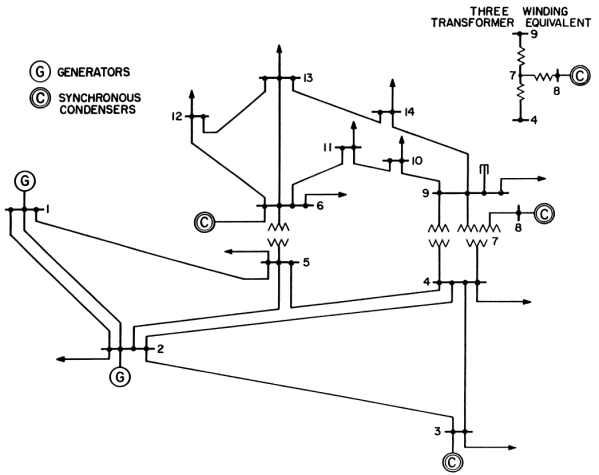
\includegraphics[width=\textwidth]{Single-line-diagram-of-IEEE-14-bus-system.png}
  \caption{IEEE 14 bus system diagram}
\end{figure}

\subsection{Initial Conditions}

The reference angle for the load flow is set at bus n°1. \\

Here are the initial conditions for each generator.

\begin{center}
\begin{tabular}{|c|c|c|c|c|}
  \hline
  Generator & P (MW) & Q (Mvar) & U (kV) & $\Theta$ (°) \\
  \hline
  1 & 232.39 & -16.55 & 73.14 & 0.00\\
  2 & 40.00 & 43.56 & 72.11 & -4.98\\
  3 & 0.00 & 25.07 & 69.69 & -12.73\\
  6 & 0.00 & 12.73 & 14.77 & -14.22\\
  8 & 0.00 & 17.62 & 15.04 & -13.36\\
  \hline
\end{tabular}
\end{center}

\subsection{Models}

\subsubsection{Synchronous Machines}

The following table recaps the modelisation of each generator.

\begin{center}
\begin{tabular}{|c|c|c|c|c|c|}
  \hline
  Generator & Windings  & Saturations & Transformer\\
  \hline
  1 & 4 & Yes & Yes\\
  2 & 4 & Yes & Yes\\
  3 & 4 & Yes & Yes\\
  6 & 3 & Yes & No\\
  8 & 3 & Yes & Yes\\
  \hline
\end{tabular}
\end{center}

All 5 machines are controlled by a proportional speed governor and a proportional voltage regulator. \\

For every machine the voltage regulator is as follows:
\begin{figure}[H]
\centering
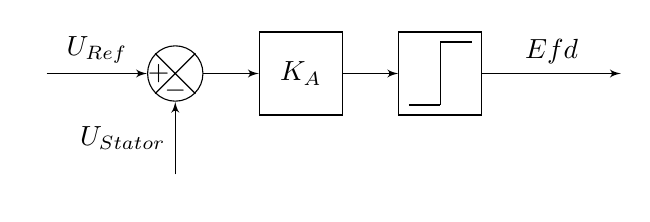
\begin{tikzpicture}
\sbEntree{E}
\sbCompSum[5]{errAVR}{E}{}{-}{+}{}
\sbRelier[$U_{Ref}$]{E}{errAVR}
\sbDecaleNoeudy[4]{errAVR}{Us}
\sbRelier[$U_{Stator}$]{Us}{errAVR}
\sbBloc{Gain}{$K_A$}{errAVR}
\sbRelier{errAVR}{Gain}
\sbBlocL{Limiter}{\tikz {\draw (-0.4,-0.4) -- (0,-0.4);\draw (0,-0.4) -- (0,0.4); \draw (0,0.4) -- (0.4,0.4); }}{Gain}
\sbSortie[5]{S}{Limiter}
\sbRelier[$Efd$]{Limiter}{S}
\end{tikzpicture}
\caption{Voltage regulator}
\end{figure}

For every machine the speed governor is as follows:
\begin{figure}[H]
\centering
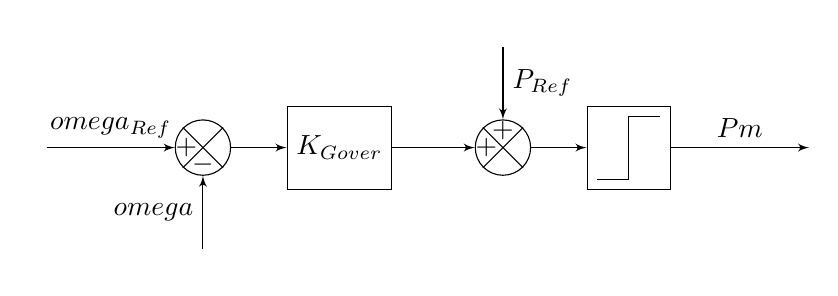
\begin{tikzpicture}
\sbEntree{E}
\sbCompSum[6]{errW}{E}{}{-}{+}{}
\sbRelier[$omega_{Ref}$]{E}{errW}
\sbDecaleNoeudy[4]{errW}{Omega}
\sbRelier[$omega$]{Omega}{errW}
\sbBloc{Gain}{$K_{Gover}$}{errW}
\sbRelier{errW}{Gain}
\sbCompSum{sumP}{Gain}{+}{}{+}{}
\sbRelier{Gain}{sumP}
\sbDecaleNoeudy[-4]{sumP}{PRef}
\sbRelier[$P_{Ref}$]{PRef}{sumP}
\sbBlocL{Limiter}{\tikz {\draw (-0.4,-0.4) -- (0,-0.4);\draw (0,-0.4) -- (0,0.4); \draw (0,0.4) -- (0.4,0.4); }}{sumP}
\sbSortie[5]{S}{Limiter}
\sbRelier[$Pm$]{Limiter}{S}
\end{tikzpicture}
\caption{Speed Governor}
\end{figure}

For every machine the voltage regulator parameters are:
\begin{center}
\begin{tabular}{l|l}
   $K_A=20$ & $Efd_{Max}=5$  \\
    & $Efd_{Min}=-5$   \\
\end{tabular}
\end{center}

For every machine the speed governor parameters are:
\begin{center}
\begin{tabular}{l|l}
   $P_{Nom}=S_{Nom_{SM}}$ & $P_{Max}=S_{Nom_{SM}}$  \\
   $K_{Gover}=5$ & $P_{Min}=0$   \\
\end{tabular}
\end{center}

\subsubsection{System reference frequency}

The system reference frequency used in every machine's model is computed as following:

\[
 \omega_{ref} = \frac{\sum_{Gen \hspace{2pt} n} H_{n} \ Snom_{n} \ \omega_{n}}{\sum_{Gen \hspace{2pt} n} H_{n} \ Snom_{n}}
\]

where $H_{n}$ is generator n inertia and $Snom_{n}$ its apparent power.
\subsubsection{Loads}

Loads follow an alpha beta dynamic behaviour, that is to say :

\[
\begin{aligned}
& P = P_{ref} (\frac{U}{U_{0}})^\alpha \\
& Q = Q_{ref} (\frac{U}{U_{0}})^\beta
\end{aligned}
\]
with $\alpha$ = 1.5 and $\beta$ = 2.5 \\
They are directly connected to the grid (no transformer included).


\subsection{Solver}
The solver used is the variable time step solver IDA with the following parameters:
\begin{itemize}
\item $Order$=2;
\item $Accuracy_{Rel}$=$10^{-4}$;
\item $Accuracy_{Abs}$=$10^{-4}$;
\end{itemize}

\subsection{Scenario}
The simulated scenario is a three-phase fault (R = $0 \ \Omega$ and X = $10^{-4} \ \Omega$) at the node 2, which corresponds to the point of connection for generator 2. The fault lasts from t = 1 s to t = 1.1 s.

\newpage
\section{Results}

For this test we focus on the response of generator 2.\\

We observe that the voltage at the node 2 falls to zero. As the voltage is zero during the fault, the generator can't evacuate its active power anymore: it falls to zero too. When the fault is cleared the voltage is restored as well as the active power, which stabilizes a few seconds after the fault clearance.\\

\begin{figure}[H]
\subfigure[Bus 2 voltage (pu)]
{%
  \begin{tikzpicture}
    \begin{axis}[height = 2in]
        \addplot[color=blue!50]
        table[x=time,y expr=\thisrow{NETWORK__BUS____2_TN_Upu_value}*69]
        {../IEEE14/IEEE14_Fault/reference/outputs/curves/curves.csv};
    \end{axis}
  \end{tikzpicture}
}
\subfigure[Reactive power (Mvar)]
{%
  \begin{tikzpicture}
    \begin{axis}[height = 2in]
        \addplot[color=blue!50]
        table[x=time, y=GEN____2_SM_generator_QGen]
        {../IEEE14/IEEE14_Fault/reference/outputs/curves/curves.csv};
    \end{axis}
  \end{tikzpicture}
}
\caption{Generator 2 response to the three-phase fault}
\end{figure}


\begin{figure}[H]
\subfigure[Omega (pu)]
{%
  \begin{tikzpicture}
    \begin{axis}[height = 2in]
        \addplot[color=blue!50]
        table[x=time, y=GEN____2_SM_generator_omegaPu]
        {../IEEE14/IEEE14_Fault/reference/outputs/curves/curves.csv};
    \end{axis}
  \end{tikzpicture}
}
\subfigure[Active power (MW)]
{%
  \begin{tikzpicture}
    \begin{axis}[height = 2in]
        \addplot[color=blue!50]
        table[x=time, y=GEN____2_SM_generator_PGen]
        {../IEEE14/IEEE14_Fault/reference/outputs/curves/curves.csv};
    \end{axis}
  \end{tikzpicture}
}
\caption{Generator 2 response to the three-phase fault}
\end{figure}

\chapter{IEEE57}

The IEEE57 bus system is a standard test case in the power system community. It represents a simple approximation of the American Electric Power system (in the U.S. Midwest) as it was in the early 1960s. The data were provided by Iraj Dabbagchi of AEP and converted into the IEEE Common Data Format by Rich Christie at the University of Washington in August 1993.

\textbf{Note. The test case is used in a modified way in this example: arbitrary dynamic data are added.}

\section{Test case description}

The IEEE 57-bus test case system has 57 buses, 7 generators, 3 shunts, 16 transformers, 63 lines and 42 loads.\\
There are three voltage levels in the test case: 69 kV, 18 kV and 13.8 kV. The outer part of the system, with the generators, corresponds to the 69 kV network. The upper inner part is the 18 kV part and the lower inner part is the 13.8 kV part.

\begin{figure}[H]
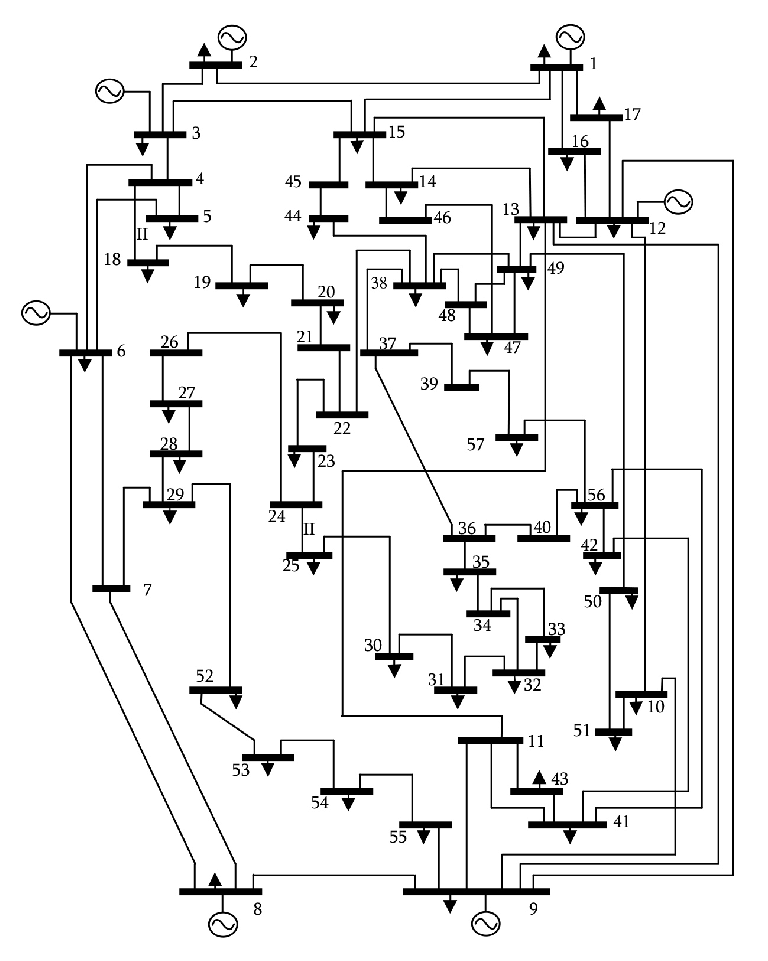
\includegraphics[scale=0.5]{IEEE57BusSystem.png}
\caption{IEEE57 system representation}
\label{circuit-1}
\end{figure}

\subsection{Models}

The generators are modeled as four windings synchronous generators models with a proportional voltage regulator and a proportional speed governor (transformers are included into the machine model; saturations are represented).

The voltage regulator is as follows:
\begin{figure}[H]
\centering
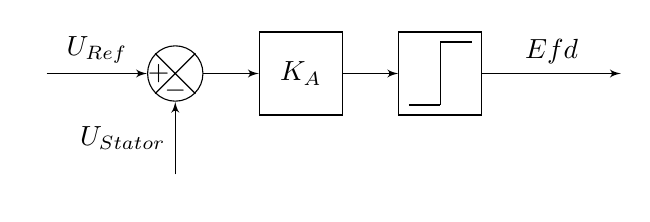
\begin{tikzpicture}
\sbEntree{E}
\sbCompSum[5]{errAVR}{E}{}{-}{+}{}
\sbRelier[$U_{Ref}$]{E}{errAVR}
\sbDecaleNoeudy[4]{errAVR}{Us}
\sbRelier[$U_{Stator}$]{Us}{errAVR}
\sbBloc{Gain}{$K_A$}{errAVR}
\sbRelier{errAVR}{Gain}
\sbBlocL{Limiter}{\tikz {\draw (-0.4,-0.4) -- (0,-0.4);\draw (0,-0.4) -- (0,0.4); \draw (0,0.4) -- (0.4,0.4); }}{Gain}
\sbSortie[5]{S}{Limiter}
\sbRelier[$Efd$]{Limiter}{S}
\end{tikzpicture}
\caption{Voltage regulator}
\end{figure}

The speed governor is as follows - omegaRef being 1 pu in this control scheme -:
\begin{figure}[H]
\centering
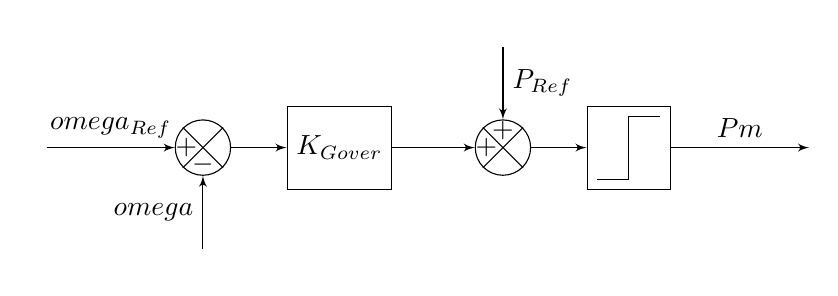
\begin{tikzpicture}
\sbEntree{E}
\sbCompSum[6]{errW}{E}{}{-}{+}{}
\sbRelier[$omega_{Ref}$]{E}{errW}
\sbDecaleNoeudy[4]{errW}{Omega}
\sbRelier[$omega$]{Omega}{errW}
\sbBloc{Gain}{$K_{Gover}$}{errW}
\sbRelier{errW}{Gain}
\sbCompSum{sumP}{Gain}{+}{}{+}{}
\sbRelier{Gain}{sumP}
\sbDecaleNoeudy[-4]{sumP}{PRef}
\sbRelier[$P_{Ref}$]{PRef}{sumP}
\sbBlocL{Limiter}{\tikz {\draw (-0.4,-0.4) -- (0,-0.4);\draw (0,-0.4) -- (0,0.4); \draw (0,0.4) -- (0.4,0.4); }}{sumP}
\sbSortie[5]{S}{Limiter}
\sbRelier[$Pm$]{Limiter}{S}
\end{tikzpicture}
\caption{Speed Governor}
\end{figure}

The loads are modeled as voltage-dependant loads:
\begin{equation*}
\begin{aligned}
& P = P_{0} * (\frac{U}{U_{0}})^\alpha \\
& Q = Q_{0} * (\frac{U}{U_{0}})^\beta
\end{aligned}
\label{Voltage-dependant load model}
\end{equation*}

The system reference frequency is calculated by the OmegaRef model using the different generators speeds.\\

All the models parameters can be viewed into the par file available in the test directory.

\subsection{Solver}
The scenario is simulated with the variable time step solver IDA using the following parameters:
\begin{itemize}
\item $Order$=2;
\item $Accuracy_{Rel}$=$10^{-4}$;
\item $Accuracy_{Abs}$=$10^{-4}$;
\end{itemize}

\subsection{Scenario}
The simulated scenario is a three-phase fault (R = $10^{-4} \ \Omega$ and X = $10^{-4} \ \Omega$) at the node 12, which corresponds to the point of connection for generator 12. The fault lasts from t = 1 s to t = 1.1 s.

\newpage
\section{Results}

For this test we focus on the responses of generators 9 and 12.\\

We observe that the voltage at the node 12 falls to zero. As the voltage is zero during the fault, the generator can't evacuate its active power anymore: it falls to zero too. When the fault is cleared the voltage is restored as well as the active power, which stabilizes a few seconds after the fault clearance.\\

\begin{figure}[H]
\subfigure[Bus 12 voltage (pu)]
{%
  \begin{tikzpicture}
    \begin{axis}[height = 2in]
        \addplot[color=blue!50]
        table[x=time,y expr=\thisrow{NETWORK__GLEN__12_TN_Upu_value}*69]
        {../IEEE57/IEEE57_Fault/reference/outputs/curves/curves.csv};
    \end{axis}
  \end{tikzpicture}
}
\subfigure[Reactive power (Mvar)]
{%
  \begin{tikzpicture}
    \begin{axis}[height = 2in]
        \addplot[color=blue!50]
        table[x=time, y=GEN___12_SM_generator_QGen]
        {../IEEE57/IEEE57_Fault/reference/outputs/curves/curves.csv};
    \end{axis}
  \end{tikzpicture}
}
\caption{Generator 12 response to the three-phase fault}
\end{figure}


\begin{figure}[H]
\subfigure[Omega (pu)]
{%
  \begin{tikzpicture}
    \begin{axis}[height = 2in]
        \addplot[color=blue!50]
        table[x=time, y=GEN___12_SM_generator_omegaPu]
        {../IEEE57/IEEE57_Fault/reference/outputs/curves/curves.csv};
    \end{axis}
  \end{tikzpicture}
}
\subfigure[Active power (MW)]
{%
  \begin{tikzpicture}
    \begin{axis}[height = 2in]
        \addplot[color=blue!50]
        table[x=time, y=GEN___12_SM_generator_PGen]
        {../IEEE57/IEEE57_Fault/reference/outputs/curves/curves.csv};
    \end{axis}
  \end{tikzpicture}
}
\caption{Generator 12 response to the three-phase fault}
\end{figure}

Generator 9 is electrically close to generator 12. When the fault is applied on node 12, the reactive power injection from generator 9 increases which contributes to limit the voltage dip on node 9. The active power injection also increases to compensate for the zero injection coming from generator 12, and oscillates during a few seconds after the fault clearance before going back to its initial value.

\begin{figure}[H]
\subfigure[Bus 9 voltage (pu)]
{%
  \begin{tikzpicture}
    \begin{axis}[height = 2in]
        \addplot[color=blue!50]
        table[x=time,y expr=\thisrow{NETWORK__SALT___9_TN_Upu_value}*69]
        {../IEEE57/IEEE57_Fault/reference/outputs/curves/curves.csv};
    \end{axis}
  \end{tikzpicture}
}
\subfigure[Reactive power (Mvar)]
{%
  \begin{tikzpicture}
    \begin{axis}[height = 2in]
        \addplot[color=blue!50]
        table[x=time, y=GEN____9_SM_generator_QGen]
        {../IEEE57/IEEE57_Fault/reference/outputs/curves/curves.csv};
    \end{axis}
  \end{tikzpicture}
}
\caption{Generator 9 response to the three-phase fault}
\end{figure}


\begin{figure}[H]
\subfigure[Omega (pu)]
{%
  \begin{tikzpicture}
    \begin{axis}[height = 2in]
        \addplot[color=blue!50]
        table[x=time, y=GEN____9_SM_generator_omegaPu]
        {../IEEE57/IEEE57_Fault/reference/outputs/curves/curves.csv};
    \end{axis}
  \end{tikzpicture}
}
\subfigure[Active power (MW)]
{%
  \begin{tikzpicture}
    \begin{axis}[height = 2in]
        \addplot[color=blue!50]
        table[x=time, y=GEN____9_SM_generator_PGen]
        {../IEEE57/IEEE57_Fault/reference/outputs/curves/curves.csv};
    \end{axis}
  \end{tikzpicture}
}
\caption{Generator 9 response to the three-phase fault}
\end{figure}

\end{document}
